\documentclass[12pt]{article}
\usepackage{amsthm,amssymb,amsfonts,amsmath,amstext,systeme}
\usepackage{graphicx,float}
\usepackage{tabularx}

\marginparwidth 0pt
\oddsidemargin -1.2 truecm
\evensidemargin  0pt 
\marginparsep 0pt
\topmargin -2.2truecm
\linespread{1}
\textheight 25.8 truecm
\textwidth 18.5 truecm
\newenvironment{remark}{\noindent{\bf Remark }}{\vspace{0mm}}
\newenvironment{remarks}{\noindent{\bf Remarks }}{\vspace{0mm}}
\newenvironment{question}{\noindent{\bf Question }}{\vspace{0mm}}
\newenvironment{questions}{\noindent{\bf Questions }}{\vspace{0mm}}
\newenvironment{note}{\noindent{\bf Note }}{\vspace{0mm}}
\newenvironment{summary}{\noindent{\bf Summary }}{\vspace{0mm}}
\newenvironment{back}{\noindent{\bf Background}}{\vspace{0mm}}
\newenvironment{conclude}{\noindent{\bf Conclusion}}{\vspace{0mm}}
\newenvironment{concludes}{\noindent{\bf Conclusions}}{\vspace{0mm}}
\newenvironment{dill}{\noindent{\bf Description of Dill's model}}{\vspace{0mm}}
\newenvironment{maths}{\noindent{\bf Mathematics needed}}{\vspace{0mm}}
\newenvironment{inst}{\noindent{\bf Instructions}}{\vspace{0mm}}
\newenvironment{notes}{\noindent{\bf Notes }}{\vspace{0mm}}
\newenvironment{theorem}{\noindent{\bf Theorem }}{\vspace{0mm}}
\newenvironment{example}{\noindent{\bf Example }}{\vspace{0mm}}
\newenvironment{examples}{\noindent{\bf Examples }}{\vspace{0mm}}
\newenvironment{topics}{\noindent{\bf Topics}}{\vspace{0mm}}
\newenvironment{outcomes}{\noindent{\bf Expected Learning Outcomes}}{\vspace{0mm}}
\newenvironment{lemma}{\noindent{\bf Lemma }}{\vspace{0mm}}
\newenvironment{solution}{\noindent{\it Solution}}{\vspace{2mm}}
\newcommand{\ds}{\displaystyle}
\newcommand{\un}{\underline}
\newcommand{\bs}{\boldsymbol}

\begin{document}

\baselineskip 18 pt
\begin{center}
	{\large \bf HKDSE MATH CORE 2020 Past Paper I}\\
	\vspace{2 mm}

\end{center}
\vspace{0.05cm}

\begin{enumerate}
	\item \textbf{HKDSE MATH CORE 2020 Past Paper I Q1}\\	
	Simplify $\dfrac{(mn^{-2})^5}{m^{-4}}$ and express your answer with positive indices. \\(3 marks)	

	\item \textbf{HKDSE MATH CORE 2020 Past Paper I Q2}\\
	Factorize
	\begin{enumerate}
		\item[(a)] $a^2 + a - 6$,
		\item[(b)] $a^4 + a^3 - 6a^2$.
	\end{enumerate}
	(3 marks)

	\item \textbf{HKDSE MATH CORE 2020 Past Paper I Q3}
	\begin{enumerate}
		\item[(a)] Round up $534.7698$ to the nearest hundred.
		\item[(b)] Round down $534.7698$ to 2 devimal places.
		\item[(c)] Round off $534.7698$ to 2 significant figures.
	\end{enumerate}
	(3 marks)

	\item \textbf{HKDSE MATH CORE 2020 Past Paper I Q4}\\
	Let $a$, $b$ and $c$ be non-zero numbers such that $\dfrac{a}{b} = \dfrac{6}{7}$ and $3a = 4c$. Find $\dfrac{b + 2c}{a + 2b}$. \\(3 marks)

	\item \textbf{HKDSE MATH CORE 2020 Past Paper I Q5}\\
	In a recruitment exercise, the number of male applicants is 28\% more than the number of femal applicants. The difference of the number of male applicants and the number of female applicants is 91. Find the number of male applicants in the recruitment exercise. \\(4 marks)

	\item \textbf{HKDSE MATH CORE 2020 Past Paper I Q6}\\
	Consider the compound inequality $$3 - x > \dfrac{7 - x}{2} \text{ or } x 5 + x > 4 \dots\dots\dots\dots\dots (*) .$$
	\begin{enumerate}
		\item[(a)] Solve (*).
		\item[(b)] Write down the greatest negative integer satisfying (*). 
	\end{enumerate}
	(4 marks)

	\item \textbf{HKDSE MATH CORE 2020 Past Paper I Q7}\\
	Let $p(x) = 4x^2 + 12x + c$, where $c$ is a constant. The equation $p(x)=0$ has equal roots. Find
	\begin{enumerate}
		\item[(a)] $c$,
		\item[(b)] the $x$-intercept(s) of the graph of $y = p(x) - 169$.
	\end{enumerate}
	(5 marks)
	
	\item \textbf{HKDSE MATH CORE 2020 Past Paper I Q8}\\
	In Figure 1, $B$ and $D$ are points lying on $AC$ and $AE$ respectively. $BE$ and $CD$ intersect at the point $F$. It is given that $AB = BE$, $BD // CE$, $\angle CAE=30^\circ$ and $\angle ADB=42^\circ$.
	\begin{figure}[H]
		\centering
		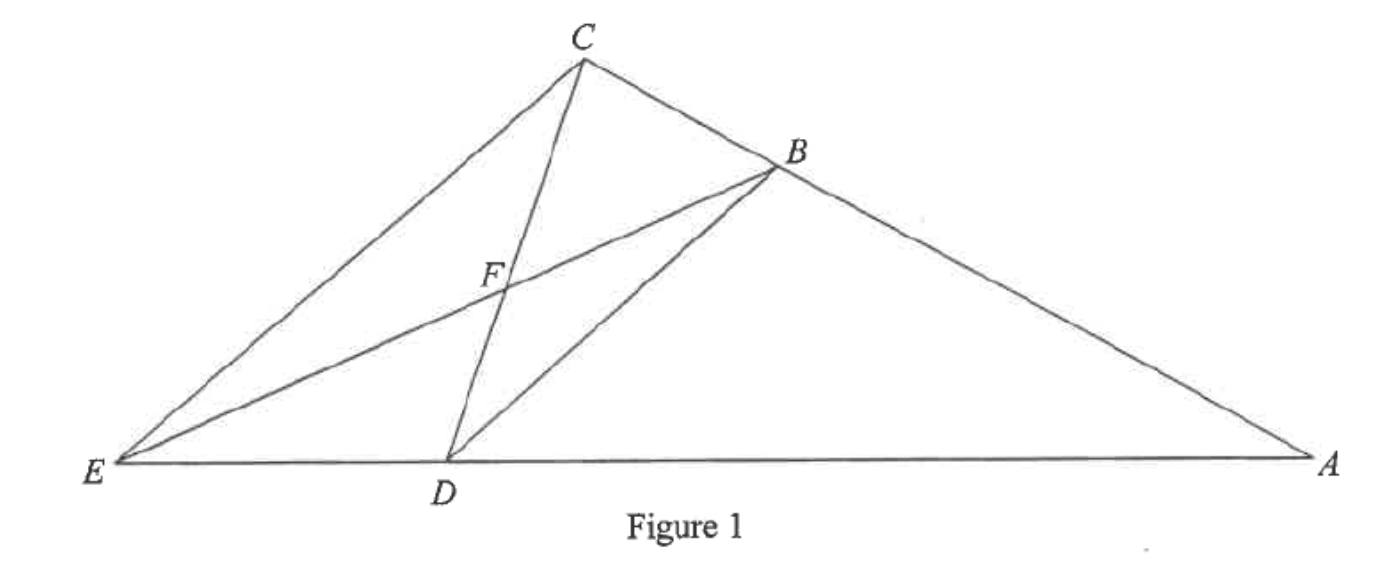
\includegraphics[width = .3\linewidth]{2020Figure1.1}
	\end{figure}
	\begin{enumerate}
		\item[(a)] Find $\angle BEC$.
		\item[(b)] Let $\angle BDC = \theta$. Express $\angle CFE$ in terms of $\theta$.
	\end{enumerate}
	(5 marks)	
	
	\item \textbf{HKDSE MATH CORE 2020 Past Paper I Q9}\\
	The table below shows the distribution of the numbers of subjects taken by a class of students.
	$$\begin{array}{|c|c|c|c|c|}
		\hline
		\text{Number of subjects taken} & 4 & 5 & 6 & 7 \\
		\hline
		\text{Number of students} & 8 & 12 & 16 & 4 \\
		\hline
	\end{array}$$
	\begin{enumerate}
		\item[(a)] Write down the mean, the median and the standard deviation of the above distribution.
		\item[(b)] A new student now joins the class. The number of subjects taken by the new student is 5. Fimd the change in the median of the distribution due to the joining of this student.
	\end{enumerate}
	(5 marks)

	\item \textbf{HKDSE MATH CORE 2020 Past Paper I Q10}\\
	The price of a brand $X$ souvenir of height $h$ cm is $\$P$. $P$ is partly constant and partly varies as $h^3$. When $h = 3$, $P = 59$ and when $h = 7$, $P = 691$.
	\begin{enumerate}
		\item[(a)] Find the price of a brand $X$ souvenir of height 4 cm. \\(4 marks)
		\item[(b)] Someone claims that the prive of a brand $X$ souvenir of height 5 cm is higher than the total prive of two bran $X$ souvenirs of height 4 cm. Is the claim correct? Explain your answer. \\(2 marks)
	\end{enumerate}

	\item \textbf{HKDSE MATH CORE 2020 Past Paper I Q11}\\
	The stem-and-leaf diagram below shows the distribution of the hourly wages (in dollars) of the workers in a group.
	\begin{table}[htbp]
		\centering
		\begin{tabular}{r|l@{\hspace{4 pt}}l@{\hspace{4 pt}}l@{\hspace{4 pt}}l@{\hspace{4 pt}}}
		   Stem (tens) & Leaf (units)     \\
			\hline
			1     & 1 2 3 3\\    
			2     & 3 3 4 5 6 9 9\\    
			3     & 1 6 7 8 8 8\\    
			4     & 2\\    
			5     & 0 $w$\\    
		\end{tabular}
	\end{table}
	It is given that the range of the above distribution is the triple of its inter-quatile range.
	\begin{enumerate}
		\item[(a)] Find $w$. \\(4 marks)
		\item[(b)] If a letter is randomly chosen from the bag, find the probability that the weight of the chosen letter is not less than the mode of the distribution. \\(2 marks)
	\end{enumerate}

	\item \textbf{HKDSE MATH CORE 2020 Past Paper I Q12}\\
	The height and the base radius of a solid right circular cone are 36 cm and 15 cm respectively. The circular cone is divided into three parts by two planes which are parallel to its base. The heights of the three parts are equal. Express, in terms of $\pi$,
	\begin{enumerate}
		\item[(a)] the volume of the middle part of the circular cone; \\(3 marks)
		\item[(b)] the curved surface area of the middle part of the circular cone. \\(3 marks)
	\end{enumerate}

	\item \textbf{HKDSE MATH CORE 2020 Past Paper I Q13}\\
	The cubic polynomial $f(x)$ is divisible by $x-1$. When $f(x)$ is divided by $x^2-1$, the remainder is $kx+8$, where $k$ is a constant.
	\begin{enumerate}
		\item[(a)] Find $k$. \\(3 marks)
		\item[(b)] It is given that $x+3$ is a factor of $f(x)$. When $f(x)$ is divided by $x$, the remainder is 24. Someone claims that all the roots of the equation $f(x) = 0$ are integers. Is the claim correct? Explain your answer. \\(5 marks)
	\end{enumerate}

	\item \textbf{HKDSE MATH CORE 2020 Past Paper I Q14}\\
	The coordinates of the points $A$ and $B$ are $(-10,0)$ and $(30, 0)$ respectively. The circle $C$ passes through $A$ and $B$. Denote the centre of $C$ by $G$. It is given that the $y$-coordinate of $G$ is $-15$.
	\begin{enumerate}
		\item[(a)] Find the equation of $C$. \\(3 marks)
		\item[(b)] The straight line $L$ passes through $B$ and $G$. Another straight line $l$ is parallel to $L$. Let $P$ be a moving point in the rectangular coordinate plane such that the perpendicular distance from $P$ to $L$ is equal to the perpendicular distance from $P$ to $l$. Denote the locus of $P$ by $\Gamma$. It is given that $\Gamma$ passes through $A$.
		\begin{enumerate}
			\item[(i)] Describe the geometric relationship between $\Gamma$ and $L$.
			\item[(ii)] Find the equation of $\Gamma$.
			\item[(iii)] Suppose that $\Gamma$ cuts $C$ at another point $H$. Someone claims that $\angle GAH < 70^\circ$. Do you agree? Explain your answer.
		\end{enumerate}
		(6 marks)
	\end{enumerate}

	\item \textbf{HKDSE MATH CORE 2020 Past Paper I Q15}\\
	In a box, there are 3 blue plates, 7 green plates and 9 purple plates. If 4 plates are randomly selected from the box at the same time, find
	\begin{enumerate}
		\item[(a)] the probability that 4 plates of the same colour are selected; \\(3 marks)
		\item[(b)] the probability that at least 2 plates of different clours are selected. \\(2 marks)
	\end{enumerate}

	\item \textbf{HKDSE MATH CORE 2020 Past Paper I Q16}\\
	The 3rd term and the 6th term of a geometric sequence are 144 and 486 respectively.
	\begin{enumerate}
		\item[(a)] Find the 1st term of the sequence. \\(2 marks) 
		\item[(b)] Find the least value of $n$ such that the sume of the first $n$ terms of the sequence is greater than $8 \times 10^{18}$. \\(3 marks)
	\end{enumerate}

	\item \textbf{HKDSE MATH CORE 2020 Past Paper I Q17}\\
	Let $g(x) = x^2 - 2kx + 2k^2 + 4$, where $k$ is a real constant.
	\begin{enumerate}
		\item[(a)] Using the method of completing the square, express, in terms of $k$, the coordinates of the vertex of the graph of $y = g(x)$. \\(2 marks)
		\item[(b)] On the same rectangular coordinate system, let $D$ and $E$ be the vertex of the graph of $y = g(x + 2)$ and the vertex of the graph of $y = -g(x -2)$ respectively. Is there a point $F$ on this rectangular coordinate system such that the coordinates of the circumentre of $\triangle DEF$ are $(0,3)$? Explain your answer. \\(4 marks)
	\end{enumerate}

	\item \textbf{HKDSE MATH CORE 2020 Past Paper I Q18}\\
	In Figure 2, $U$, $V$ and $W$ are points lying on a circle. Denote the circle by $C$. $TU$ is the tangent to $C$ at $U$ such that $TVW$ is a straight line.
	\begin{figure}[H]
		\centering
		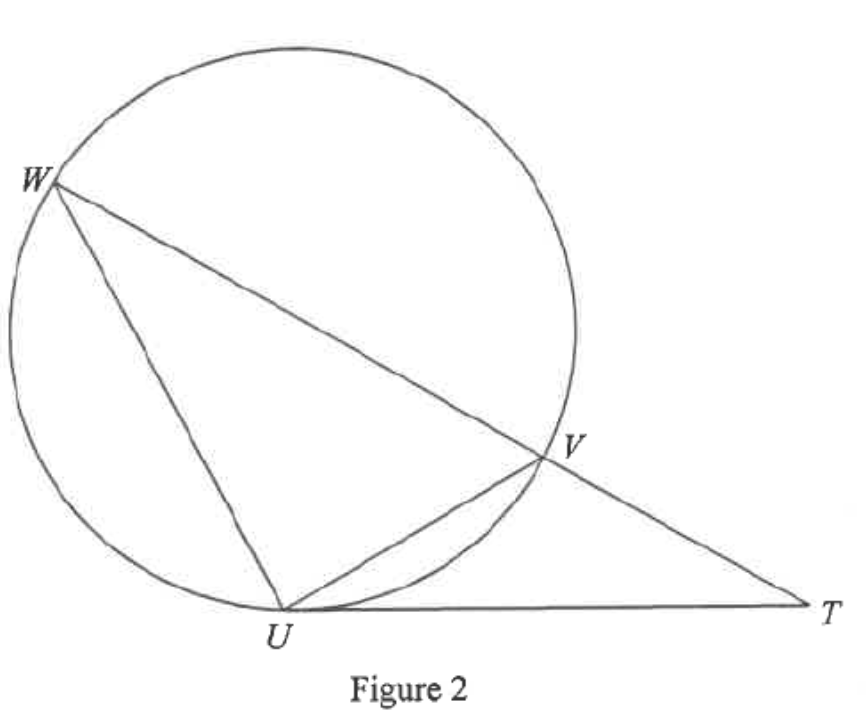
\includegraphics[width = .3\linewidth]{2020Figure1.2}
	\end{figure}
	\begin{enumerate}
		\item[(a)] Prove that $\triangle UTV \sim \triangle WTU$. \\(2 marks)
		\item[(b)] It is given that $VW$ is a diameter of $C$. Suppose that $TU = 780$ cm and $TV = 325$ cm.
		\begin{enumerate}
			\item[(i)] Express the circumference of $C$ in terms of $\pi$.
			\item[(ii)] Someone claims that the perimeter of $\triangle UVW$ exceed 35 m. Do you agree? Explain your answer.
		\end{enumerate}
		(5 marks)
	\end{enumerate}

	\item \textbf{HKDSE MATH CORE 2020 Past Paper I Q19}\\
	$PQRS$ is a quadrilateral paper card, where $PQ = 60$ cm, $PS = 40$ cm, $\angle PQR = 30^\circ$, $\angle PRQ = 55^\circ$ and $\angle QPS = 120^\circ$. The paper card is held with $QR$ on the horizontal ground as shown in Figure 3.	
	\begin{figure}[H]
		\centering
		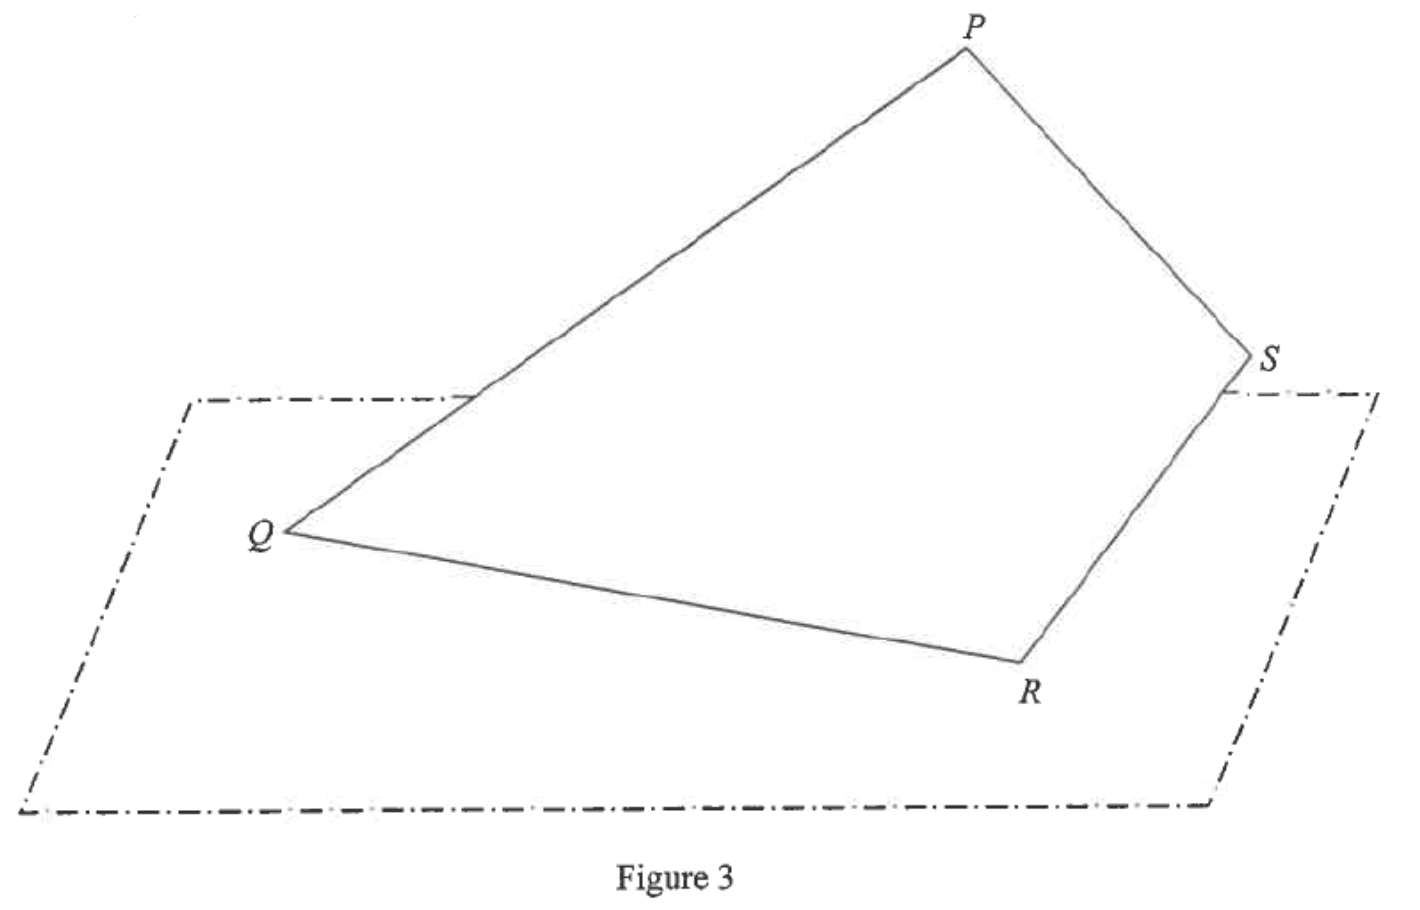
\includegraphics[width = .3\linewidth]{2020Figure1.3}
	\end{figure}
	\begin{enumerate}
		\item[(a)] Find the length of $RS$. \\(3 marks)
		\item[(b)] Find the area of the paper card. \\(3 marks)
		\item[(c)] It is given that the angle between the paper card and the horizontal ground is $32^\circ$.
		\begin{enumerate}
			\item[(i)] Find the shortest distance from $P$ to the horizontal ground.
			\item[(ii)] A student claims that the angle between $RS$ and the horizontal ground is atmost $20^\circ$. Is the claim correct? Explain your answer.
		\end{enumerate}
		(7 marks)
	\end{enumerate}


\end{enumerate}
\end{document}